\chapter{結論與未來展望}
\section{結論}
\indent
本論文在基於呂昭陞論文提出的Xpath撰寫樣式的使用前提下,
為減少尋找適合元件定位條件的時間,而提出利用HTML文本比對的瀏覽器擴充元件找出適合元件定位的條件。

使用者一般在查找變化時,通常都會使用瀏覽器中的Developer Tools來觀察元件是否有淺紫背景框的,
但這個方法較慢又較容易忽略一些更好當成Xpath條件的變化。
此擴充元件透過HTML文本比對,將有變化的元件列舉出來,讓使用者可以直接透過結果挑選適合的變化加入Xpath的條件中,
無論是無相關經驗或已經有一定基礎的測試人員使用Developer Tools配合此擴充元件查找變化,
相較於只用Developer Tools,時間減少20~30\%左右,尤其無相關經驗的測試人員減少的時間會更多一些。
由此可知,透過Developer Tools加上擴充元件的輔助可以降低設計Xpath所花用時間,提高撰寫測試腳本的效率。

\section{未來方向}
\indent
本論文提出之HTML文本比對工具仍有待改善之處,以下將分為五點說明:

\begin{itemize}
\item\textbf{比較節點相異等級之演算法:}

本論文使用的比較文本程式,在計算節點相異的等級,
有分成"IDENTICAL"、"SAME BUT DIFFERENT"和"NOT THE SAME NODE"三種類型。
用於判斷的演算法是使用權重的方式來看各個屬性的相異性來給他們相對應的權重,
但若使用這種方法的時候,因為在判定"SAME BUT DIFFERENT"和"NOT THE SAME NODE"這兩種類型時,
沒辦法精準的判定是不是類型等級,
像是圖\ref{f5.1}中以我們使用者的角度會知道它是id="456"的節點刪除,
但以原本的演算法會因為節點等級,
而判斷成id="456"的元件修改成id="789"的元件,原本id="789"的元件則會被刪除。
若能調整判斷節點的演算法使它更能趨近使用者的結果,最後輸出的節點變化類型也會更精確。

\indent
\begin{figure}[H]
    \centering
    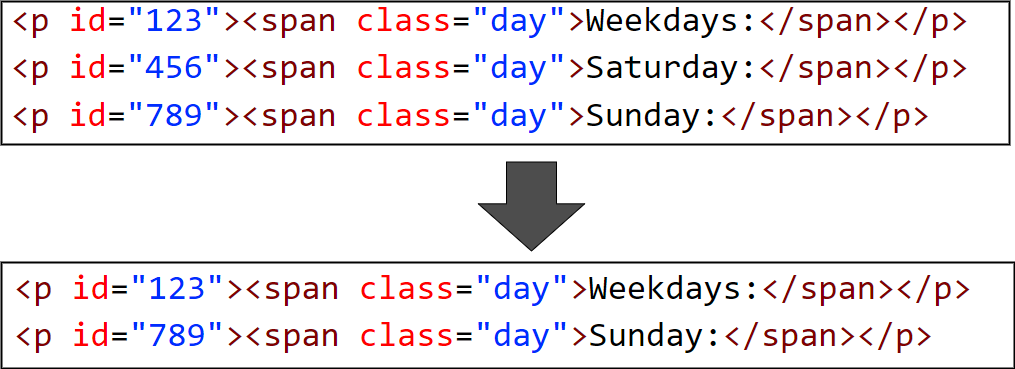
\includegraphics[width=0.8\textwidth]{picture/ch-5 Heuristic_improve.png}
    \caption{比較節點相異等級之情境}
    \label{f5.1}
\end{figure}

\item\textbf{比對相異之元件自動跳轉到Develope Tool中Element頁面並標記}

此工具在顯示結果時,僅只有告訴使用者變化元件的路徑,
使用者必須照著路徑一個一個慢慢找出找出變化的元件,
或透過畫面上的元件變化直接用Developer Tools中"Inspect Element"的功能找出元件後再查看是不是比較結果中的元件,
若以上述的兩種作法操作,使用速度及方便度會降低。
若在查看比較結果時,
可以讓使用者直接跳轉到Developer Tools中Element頁面上的該元件,
會讓使用者可以快速的觀察出變化並設計Xpath表達式。

\item\textbf{比對結果過濾功能新增:}

在目前此工具建立了三個可以過濾結果的選項,
可以依照使用者的當下的情況來過濾掉不需要的結果,
從而可以更快速地找出Xpath表達式中的條件設定,
若增加更多可刪選的情況,便可以進一步地把無用的結果篩選掉。

\item\textbf{紀錄多個狀態的HTML文本:}

目前的設計僅能儲存開始計時前和計時後的兩個文本;
若能增加暫存功能,
能記錄多個狀態的文本並且挑選其中兩個狀態的文本來進行比對,
也會加快使用者在操作的方便性,
而不用因為已經解析過當下的文本狀態,需要等待計時器和程式的運行時間,


\item\textbf{UI/UX介面美化及更人性化:}

在設計UI介面時,僅用基本的顏色和元件來進行簡單的操作;
而UX介面是以較大的字樣以及元件為主軸,會造成頁面上會常常操作到滾輪來移動畫面。
若在頁面上加上分頁或下拉選單...等等可以隱藏部分元件的設計,
可以增加頁面的乾淨程度,並更利於使用者操作。

\end{itemize}